\chapter{Formalism \& numerical methods}

Despite the deuteron problem was solved long time ago, I will describe it briefly 
in order to introduce the notation and formalism. 
With that, for more complex 3N case only slight 
extension will be needed.

In order to calculate any observable for the deuteron photodisintegration,
one has to find a nuclear matrix elements:

% \begin{equation}
%     N^\mu = \langle \Psi_f \vec{P_f} \mid \frac{1}{e}J^\mu(0) \mid \Psi_i \vec{P_i} \rangle =
%     \langle p' (l's')j'm_j't'm_t' \vec{P_f} \mid J^\mu \mid \phi_d m_d \vec{P}_i \rangle, 
%     \label{main}
% \end{equation}
\begin{equation}
    N^\mu = \langle \Psi_{final} \mid J^\mu \mid \Psi_{initial} \rangle, 
    \label{main}
\end{equation}
with two-nucleon wave function of the initial state $\Psi_{initial}  = \Psi_{deuteron}$;
two-nucleon wave function of the final scattering state $\Psi_{final}$ 
and a four-vector current operator $J^\mu$ which acts between initial and final 
two-nucleon states. In following I describe how to get that quantities.


% $\vec{P_i}$($\vec{P_f}$) is an initial (final) total 2N m\vec{p}omentum.

% One can introduce relative and total momenta for 2 nucleons:

% \begin{eqnarray}
    %     \vec{p} &=& \frac{1}{2} (\vec{p}_1 - \vec{p}_2)\\
    %     \vec{\mathcal{P}} &=& \vec{p}_1 + \vec{p}_2\\
    %     \pvec{p} &=& \frac{1}{2} (\pvec{p}_1^\prime - \pvec{p}_2^\prime)\\
    %     \pvec{\mathcal{P}}^\prime &=& \pvec{p}_1^\prime + \pvec{p}_2^\prime,
    % \end{eqnarray}
    % where $\vec{p}_1$($\pvec{p}_1^\prime$) and $\vec{p}_2$($\pvec{p}_2^\prime$) are
    % initial(final) momenta of the first and second nucleons.
\section{Deuteron bound state}
    \label{sec:deut_bound}

    Let's find a deuteron bound state wave function $\ket{\phi_d}$. 
    The time-independent Schr\"{o}dinger
    equation for two particles expresses as:

    \begin{equation}
        (H_0 + V) \ket{\phi_d}  = E_d \ket{\phi_d},
        \label{shrod_bound}
    \end{equation}
    with a kinetic energy $H_0$ and potential $V$. 
    The kinetic energy $H_0$ can be represented in terms of  relative and total momenta
    of the particles:

    \begin{equation}
        H_0 = \frac{\vec{p}_1^2}{2m_1} + \frac{\vec{p}_2^2}{2m_2} = 
        \frac{\vec{p}^2}{2\mu} + \frac{\vec{\mathcal{P}}^2}{2M}, 
    \end{equation}
    where relative and total momenta are defined as follows:

    \begin{eqnarray}
        \vec{p} &=& \frac{(m_1\vec{p}_1 - m_2\vec{p}_2)}{m_1 + m_2}\\
        \vec{\mathcal{P}} &=& \vec{p}_1 + \vec{p}_2
    \end{eqnarray}
    $M = m_1 + m_2$ is a total mass, $\mu = \frac{m_1m_2}{M}$ is a relative mass of two nucleons and 
    $\vec{p_i}$ is a momentum of i-th particle.

    Potential $V$ is assumed to depend on the relative degrees of freedom only, so
    \eq{shrod_bound} may be decomposed into two separated equations:

    \begin{eqnarray}
        &\frac{\vec{p}^2}{2\mu} \langle \vec{p} \mid \Psi_{int} \rangle +
        \langle \vec{p} \mid V \mid \Psi_{int} \rangle = 
        (E_d - E)\langle \vec{p} \mid \Psi_{int} \rangle \label{se1}\\
        &\frac{\vec{\mathcal{P}}^2}{2M} \langle \mathcal{P} \mid \Psi \rangle = 
        E\langle \mathcal{P} \mid \Psi \rangle \label{se2},
    \end{eqnarray}
    with $\matrixel{\vec{p},\vec{\mathcal{P}}}{H_0}{\phi_d} = \frac{\vec{p}^2}{2\mu} \braket{\vec{p}}{\Psi_{int}} +
    \frac{\vec{\mathcal{P}}^2}{2M} \braket {\mathcal{P}} {\Psi} $. So $\Psi$ is a component 
    of total wave function, which reflects a deuteron as a single object with momentum $\vec{\mathcal{P}}$
    while $\Psi_{int}$ is an internal wave function describing interaction between nucleons.
    Basis state $\ket{\vec{p}}$  obeys a completeness
    equation:

    \begin{equation}
        \int d^3\vec{p} \ket{\vec{p}} \bra{\vec{p}}   = \mathbb{1}
        \label{completness}
    \end{equation}

    Eq.(\ref{se1}) is basically a Schr\"{o}dinger equation for one particle with mass $\mu$
    in potential $V$ 
    and Eq.(\ref{se2}) can be regarded as a Schr\"{o}dinger equation for particle with mass $M$ in 
    a free motion. Assuming that deuteron is at rest ($E_{c.m.} = 0$) we can stick 
    to the Eq.(\ref{se1}) only. Using completeness relation \ref{completness} we get:

    \begin{equation}
        \frac{\vec{p}^2}{2\mu} \langle \vec{p} \mid \Psi_{int} \rangle +
        \int d \pvec{p} \langle \vec{p} \mid V \mid \pvec{p} \rangle
        \langle \pvec{p} \mid \Psi_{int} \rangle = 
        E_d \langle \vec{p} \mid \Psi_{int} \rangle
        \label{shrod_old}
    \end{equation}

    Working in 3 dimensional space  is difficult (especially numerically)
    so I follow a standard path and introduce the partial-wave decomposed representation (PWD) 
    of the momentum state, adding spin and isospin degrees of freedom in the following form:

    \begin{equation}
        \ket{p \alpha} \equiv \ket{p (ls) j m_j}  \ket{t m_t},
        \label{pwmain}
    \end{equation}
    where quantum numbers l, s, j, t are orbital angular momentum, total spin,
    total angular momentum and total isospin respectively. $m_j$ and $m_t$ are 
    total angular momentum and isospin projections, respectively.


    States $\ket{p (ls) j m_j}$ can be further decomposed to 
    the main basis states than it is in (\ref{pwmain}), separating spin part as 
    
    \begin{equation}
        \ket{p (ls) j m_j} = \sum_{m_l} c(lsj;m_l, m_j\!-\!m_l, m_j) \ket{p l m_l}
        \ket{s~m_j\!-\!m_l}.
        \label{full_decomp}
    \end{equation}

    Spin(isospin) states can be further represented via single-nucleon spin(isospin) states:

    \begin{equation}
        \ket{s m_s} = \sum_{m_1} c(\frac{1}{2}\frac{1}{2}s;m_1, m_s\!-\!m_1, m_s)
        \ket{\frac{1}{2} m_1}
        \ket{\frac{1}{2} m_s\!-\!m_1},
        \label{spin_decomp}
    \end{equation}

    \begin{equation}
        \ket{t m_t} = \sum_{\nu_1} c(\frac{1}{2}\frac{1}{2}t;\nu_1, m_t\!-\!\nu_1, m_t)
        \ket{\frac{1}{2} \nu_1}
        \ket{\frac{1}{2} m_t\!-\!\nu_1}.
        \label{isospin_decomp}
    \end{equation}

    In Eqs.(\ref{full_decomp}) -(\ref{isospin_decomp}),  $c(...)$ are Clebsh-Gordon coefficients.
    Nucleons are spin $\frac{1}{2}$ particles, and also we treat proton and neutron as 
    the same particle in different 
    isospin states, so that isospin $\nu_1 = \frac{1}{2}$ stands for proton and $\nu_1 = -\frac{1}{2}$ for neutron.

    The states $\mid p l m_l \rangle$ from Eq.(\ref{full_decomp}) are orthogonal
    
    \begin{equation}
        \langle p^\prime l^\prime m_l^\prime \mid p l m_l \rangle = 
        \frac{\delta(p - p^\prime)}{p^2} \delta_{ll^\prime}\delta_{m_l m_l^\prime}
    \end{equation}
    and also satisfy the completeness relation:

    \begin{equation}
        \sum_{l=0}^\infty \sum_{m_l=-l}^l \int dp p^2 \mid plm_l \rangle \langle plm_l \mid = \mathbb{1}
    \end{equation}


    Projection of $\bra{\pvec{p}}$ states to $\ket{plm_l}$ leads to

    \begin{equation}
        \braket{\pvec{p}}{plm_l} = 
        \frac{\delta ( \abs{\pvec{p}} - p)}{p^2} Y _{l m_l}(\hat{p}^\prime),
    \end{equation}
    where $Y _{l m_l}(\hat{p}^\prime)$ is a spherical harmonic and 'hat' denotes a unit vector $\hat{X}$ in 
    direction of $\vec{X}$. So for the momentum vector:

    \begin{equation}
        \vec{p} \equiv |\vec{p}| \hat{p} \equiv p \hat{p}. 
        \label{hat}
    \end{equation}

    Nucleons are fermions so exchanging them leads to antisymmetry of the
    wave function. In PWD it results in additional requirement on allowed quantum numbers which
    is:

    \begin{equation}
        (-1)^{l+s+t} = -1.
        \label{parity}
    \end{equation}

    In general, nuclear NN force conserves spin, parity and charge so

    \begin{equation}
        \matrixel*{p^\prime\alpha^\prime}{V}{p\alpha} = \delta_{jj'}\delta_{mm'}\delta_{tt'}\delta_{m_tm_{t'}}
        \delta_{ss'}V^{sjtm_t}_{l'l}(p',p)
        \label{conservation}
    \end{equation}
    which introduces restrictions for particular sets of quantum numbers.
    Strong interaction allows for change of the orbital angular momenta $l = j \pm 1,~l'=j'\pm1$.
    The channels, where $l \neq l'$
    are coupled and for the deuteron bound state 
    one can find only one possible PWD state combination:
    two coupled channels 
    which are commonly denoted as $^3S_1$ and $^3D_1$ (the naming stands for $^{2s+1}l_j$). They correspond 
    to $l=0$ and $l=2$ respectively (with $s = j = 1$ and $t = m_t = 0$). 
    We will call wave functions for these channels as $\phi_l(p)$ with $l=0,2$, such that:

    % Taking into account Eq.(\ref{parity}), one can find only one possible PWD state combination for 
    % the deuteron bound state(under ... experimental evidence): 2 coupled channels for l=0,2; s=1; j=1 and $t = m_t = 0$. 
    % These 2 channels are usually denoted as $^3S_1$ and $^3D_1$ and
    % corresponding wave functions are $\phi_0(p)$ and $\phi_2(p)$:
    
    \begin{equation}
        \phi_l(p) = \bra{p (ls) j m_j}\braket{t m_t}{\Psi_{int}} = \bra{p(l1)1m_d} \braket{00}{\Psi_{int}}; l=0,2.
        \label{deut_waves}
    \end{equation}

    In that new basis Eq.(\ref{shrod_old}) takes a form of two coupled equations:

    \begin{equation}
        \frac{\vec{p}^2}{2\mu} \phi_l(p) +
        \sum_{l^\prime =0,2} \int d p^\prime p^{\prime 2} 
        \bra{p(l1)1m_d} \matrixel{00}{V}{00} \ket{p^\prime(l^\prime1)1m_d}
        % \langle plm_l \mid V \mid p^\prime l^\prime m_l^\prime  \rangle
        \phi_{l^\prime}(p^\prime) = 
        E_d \phi_l(p),
        \label{integral}
    \end{equation}
    for $l=0,2$. In case one does not have a matrix elements for the potential 
    $\langle plm_l \mid V \mid p^\prime l^\prime m_l^\prime  \rangle$ in analytical form,
    but only numerical values for some grid of points, 
    there is still one complication in the Eq.(\ref{integral}) - integration, which has to be discretized.
    In order to get rid of the integral I use a Gaussian quadrature 
    method of numerical integration \cite{jacobi1826ueber}.
    It allows to replace an integral by the weighted sum:
        $\int_a^b f(x)dx = \sum_{i=1}^n \omega_i f(x_i)$
    In current work I used $N=72$ points in the interval from $0$ to \SI{50}{fm^{-1}}. 
    Using this method, Eq.(\ref{integral}) becomes  

    
    \begin{equation}
        \frac{p_i^2}{2\mu} \phi_l(p_i) +
        \sum_{l^\prime =0,2}\sum_{j =0}^{N_P}  \omega_j p^{2}_j 
        \bra{p_i(l1)1m_d} \matrixel{00}{V}{00} \ket{p_j(l^\prime1)1m_d}
        % \langle p_jlm_l \mid V \mid p^\prime_j l^\prime m_l^\prime  \rangle
        \phi_{l^\prime}(p_j) = 
        E_d \phi_l(p_i).
        \label{integral2}
    \end{equation}

    In practical computations, the same grid points $p_i$ and $p_j$ are used in order
    optimize computational time. 
    I solve this equation as an eigenvalue problem $M\Psi = E_d \Psi$ and
    in that way
    find simultaneously wave function values in grid of $p$ points and binding energy $E_d$. 
    The binding energy $E_d$ calculated with potentials of different chiral orders 
    is presented in Fig.~\ref{bind}.

    \begin{figure}[h]
        \begin{center}
            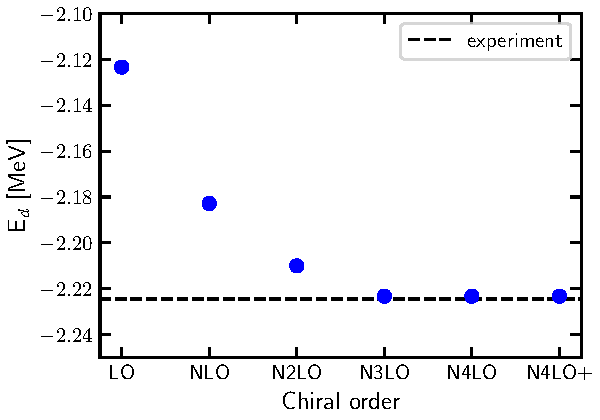
\includegraphics[width=0.65\textwidth]{Figures_De/Binding_energy.pdf}
        \end{center}
        \caption{Deuteron binding energy calculated using the chiral \gls{sms} potential
        at different chiral orders as a mean value over all cutoffs.
        Error bands represent a spread the calculated binding energy with respect to
        the cutoff parameter $\Lambda$ (minimal and maximal values).
        Experimental data is taken from \cite{VANDERLEUN1982261}}
        \label{bind}
    \end{figure}

    An example of such wave functions is demonstrated in \fig{wave_func}. The left pane demonstrate
    a wave function for $l=0$ - $^3S_1$ while the right one - for $l=2$ - $^3D_1$. Both 
    plots consist of the curves for different cutoff values and using the chiral \gls{sms} potential at \gls{n4lo+}.
    The small deviation between lines show that cutoff dependency is rather weak at this stage
    and further discrepancies connected to the value of $\Lambda$ may appear in other components.  

    \begin{figure}[h]
        \begin{center}
            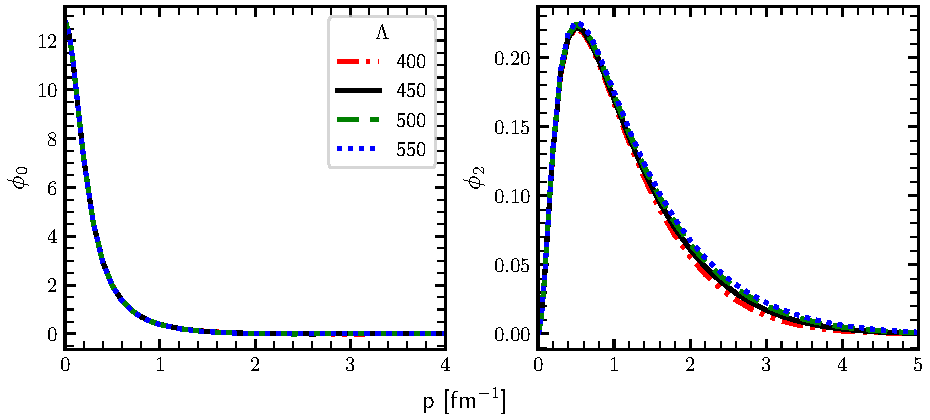
\includegraphics[width=0.85\textwidth]{Figures_De/Wave_function_cutoff.pdf}
        \end{center}
        \caption{Wave function $\phi_l$ for l=0 ($^3S_1$ partial wave)(left) and l=2 ($^3D_1$) (right).
        Each curve shows results obtained with different values of the cutoff parameter $\Lambda$, 
        results have been obtained using the chiral \gls{sms} potential at \gls{n4lo+}.}
        \label{wave_func}
    \end{figure}

\section{2N scattering state}

\subsection{The Lippmann-Schwinger equation}
    % Let us consider a two-nucleon scattering state $\mid \Psi _f \rangle$, It fulfills
    % a Schr\"{o}dinger equation

    % \begin{equation}
    %     (H_0 + V) \mid \Psi _f \rangle = E \mid \Psi _f \rangle,
    %     \label{schrod_scatt}
    % \end{equation}
    % with $H_0 = \frac{\vec{p}^2}{m}$ and $E > 0$.

    % Solution to the Eq.(\ref{schrod_scatt}) can be presented in the form:

    % \begin{equation}
    %     \mid \Psi _f \rangle = \mid \Psi _0 \rangle + \frac{1}{E - H_0 + i \epsilon} V \mid \Psi _f \rangle
    % \end{equation}

    Let us start from the time-independent formulation of the scattering process.
    In such a case Hamiltonian is:

    \begin{equation}
        H = H_0 + V,
    \end{equation}
    where again $H_0$ is a kinetic energy operator $H_0 = \frac{\vec{p}^2}{2m}$ 
    and $V$ is a nucleon-nucleon interaction.
    For a free particle motion, $V$ will be absent and we will denote a corresponding energy eigenstate as
    a free particle state $\mid \vec{p}_0 \rangle$.
    The scattering state $\ket{\psi}$ fulfills similar Schr\"{o}dinger equation as 
    $\mid \vec{p}_0 \rangle$, with the same energy eigenvalue, but with potential presented:
    
    % , the eigenstate will differ from $\ket{\phi_l}$,
    % but in case of elastic scattering (which we are interested in) the energy eigenvalue $E$ should be the same.

    % So these two states fulfill Schr\"{o}dinger equations for such scattering process:

    \begin{equation}
        \begin{cases}
            H_0 \mid \vec{p} \rangle &= E \mid \vec{p} \rangle \\
            (H_0 + V) \mid \psi \rangle &= E \mid \psi \rangle
        \end{cases}
        \label{system}
    \end{equation}

    We are interested in solution for Eq.~(\ref{system}), so that 
    $\mid \psi \rangle \rightarrow \mid \vec{p} \rangle$ as $V \rightarrow 0$
    and both $\mid \psi \rangle$ and $\mid \vec{p} \rangle$ have the same energy eigenvalues E.
    As we have scattering process, the energy spectra for both operators $H_0$ and $H_0 + V$
    are continuous. 

    From Eq.~(\ref{system}) follows that

    \begin{equation}
        \mid \psi \rangle = \frac{1}{E - H_0}V \mid \psi \rangle +  \mid \vec{p} \rangle,
        \label{psieq}
    \end{equation}
    % where $\mid \vec{p} \rangle$ is a solution to the
    % free-particle Schr\"{o}dinger equation
    % \begin{equation}
    %     H_0 \ket{\vec{p}} =  E  \ket{\vec{p}},
    % \end{equation}
    % with same energy eigenvalue\cite{Sakurai}.
    % was added artificially in order to satisfy a criterion mentioned above 
    % and following the logic from . 
    % In addition, it 
    which guarantees that
     application of the operator $(E -H_0)$ to the 
    (\ref{psieq}) results in the second equation from the set (\ref{system}).
    % Also, \eq{psieq} for $V \rightarrow 0$ becomes $\mid \psi \rangle = \mid \vec{p} \rangle$


    In order to deal with a singular operator $\frac{1}{E - H_0}$ in \eq{psieq}, the well-known
    technique is to make such an operator complex by adding small imaginary number to the denominator
    so Eq.(\ref{psieq}) becomes
    % making it  $\frac{1}{E + i\epsilon - H_0}$.

    \begin{equation}
        \ket{\psi} = G_0(E \pm i\epsilon)V \mid \psi \rangle +  \mid \vec{p} \rangle,
        \label{lse}
    \end{equation}
    where $G_0$ is a free propagator:

    \begin{equation}
        G_0(z) = \frac{1}{z - H_0}.
        \label{g0}
    \end{equation}

    Solution with $G_0(E - i\epsilon)$ corresponds to the incoming spherical wave,
    while $G_0(E + i\epsilon)$ - to the outgoing one. Since we are interested in the final scattering
    state, only the $(+)$ sign survives.
    
    Eq.~(\ref{lse}) is known as the Lippmann-Schwinger equation (LSE).
    Defining the transition operator $t$:

    \begin{equation}
        t \ket{\vec{p}} = V \ket{\psi}
        \label{t-op}
    \end{equation}
    we can rewrite it as 

    \begin{equation}
        \ket{\psi} = (1 + G_0(E + i\epsilon) t)  \ket {\vec{p}}
        \label{psi_toper}
    \end{equation}

    With substitution of \eq{lse} into \eq{t-op} we can find
    an explicit form of the $t$ operator:

    \begin{eqnarray}
        t \ket{\vec{p}} = V G_0(E + i\epsilon)V \mid \psi \rangle +  V \mid \vec{p} \rangle = \nonumber\\
        = V G_0(E + i\epsilon) t \ket{\vec{p}} +  V \mid \vec{p} \rangle
        \label{top2}
    \end{eqnarray}

    Getting rid off the initial state $\ket{\vec{p}}$ in the \eq{top2} we can get the LSE
    for the transition operator in the iterative form:

    \begin{eqnarray}
        t = V + V G_0 t = \nonumber\\
        = V + V G_0 V + V G_0 V G_0V + ...,
        \label{lse_gen}
    \end{eqnarray}
    which constitutes an infinite series of subsequent NN interactions and free propagators of nucleons.

    In the partial-wave representation, the LSE \eq{top2} expresses as:
    \begin{multline}
        \bra{p^\prime (l^\prime s^\prime)j'm_{j'}}\matrixel{t' m_{t'}}{t(E)}{t m_t}\ket{p (l s)jm_{j}} = 
        \bra{p^\prime (l^\prime s^\prime)j'm_{j'}}\matrixel{t' m_{t'}}{V}{t m_t}\ket{p (l s)jm_{j}} + \\
        +\sum_{\alpha^{\prime\prime}} \int_0^\infty dp^{\prime \prime} p^{\prime \prime 2}
        \bra{p^\prime (l^\prime s^\prime)j'm_{j'}}\matrixel{t' m_{t'}}{V}
        {t'' m_{t''}}\ket{p'' (l'' s'')j''m_{j''}} \\
        \cross \frac{1}{E + i\epsilon - p^{\prime \prime 2}/m}
        \bra{p'' (l'' s'')j''m_{j''}}\matrixel{t'' m_{t''}}{t(E)}{t m_t}\ket{p (l s)jm_{j}},
        \label{lse_pwd}
    \end{multline}
    which after using symmetries of potential matrix elements (\ref{conservation}) reduces to
    
    \begin{multline}
        \matrixel{p^\prime (l^\prime s^\prime)jt}{t(E)}{p(ls)jt} = 
        \matrixel{p^\prime (l^\prime s)jt}{V}{p(ls)jt} + \\
        +\sum_{l^{\prime\prime}} \int_0^\infty dp^{\prime \prime} p^{\prime \prime 2}
        \matrixel{p^\prime (l^\prime s)jt}{V}{p^{\prime\prime}(l^{\prime\prime} s)jt} \\
        \cross \frac{1}{E + i\epsilon - p^{\prime \prime 2}/m}
        \matrixel{p^{\prime \prime} (l^{\prime \prime} s)jt}{t(E)}{p(l s)jt}.      
        \label{lse_pwd_reduced}
    \end{multline}

    I solve \eq{lse_pwd_reduced} numerically, which again requires discretisation
    and therefor leads to set of linear equations.
    Finally, using \eq{psi_toper} and denoting the momentum state of two nucleons
    with spin projections $m_p$ and $m_n$ as $\bra{\phi m_p m_n}$, we can write \eq{main} as
    
    \begin{equation}
        N^\mu = \bra{\phi m_p m_n} (1 + G_0(E + i\epsilon) t) \frac{1}{e}J^\mu(0) \mid \Psi_i \vec{P_i} \rangle
        \label{main_top}
    \end{equation}

    %TODO: rewrite everything in \phi m_d m_n
    
\section{3N bound state}

    The 3N bound state is described by the Schr\"{o}dinger equation for 3N system
    and its total wave function obeys the following equation:

    \begin{equation}
        \ket{\Psi} = G_0(E+i\epsilon)\sum_{j=1}^3 (V_j + V_4^j) \ket{\Psi},
        \label{psi3_total}
    \end{equation}
    where $G_0$ is a free propagator from \eq{g0}, $V_j$ - is a two-body potential
    acting between nucleons $k$ and $l$ (j, k and l - numerate nucleons, $j,k,l \in {1,2,3}$ and $j \neq k \neq l$)
    and $V_4^j$ is a component of three-body potential $V_4 = \sum_{j=1}^3 V_4^j$
    symmetrical under exchange of nucleons $k$ and $l$,
    E - is a binding energy.

    \eq{psi3_total} can be split into 3 independent equations for
    so-called Faddeev components $\ket{\psi_j}$

    \begin{equation}
        \ket{\Psi} = \sum_{j=1}^3 \ket{\psi_j},
        \label{faddeev_comps}
    \end{equation}
    which fulfills separately

    \begin{equation}
        \ket{\psi_j} = G_0(E+i\epsilon)(V_j + V_4^j) \ket{\Psi}.
        \label{psi3_component}
    \end{equation}

    Next, I introduce a permutation operator P, which is a combination
    of operators $P_{jk}$:
    
    \begin{equation}
        P = P_{12}P_{23} + P_{13}P_{32}.
        \label{permutation}
    \end{equation}

    The operator component $P_{jk}$ acting on the state interchange the momenta and  
    quantum numbers of the nucleons $j$ and $k$.

    Using definitions \ref{permutation} and \ref{faddeev_comps},
    one can rewrite \eq{psi3_component} as:

    \begin{equation}
        \ket{\psi_j} = G_0(E+i\epsilon)t_j P \ket{\psi_j} + 
        (1 + G_0(E+i\epsilon)t_j)G_0(E+i\epsilon)V_4^j(1+P)\ket{\psi_j},
        \label{fadeed_lse}
    \end{equation}
    where $t_j$ is a two-body t-operator which obeys \eq{top2} for corresponding 
    two-body potential $V_j$.

The partial wave representation of the \eq{fadeed_lse} is obtained using
following states:

\begin{equation}
    \ket{p,q,\alpha_{J,M_J}} = \ket{p,q,(ls)j, (\lambda, \frac{1}{2})I(jI)JM;(t\frac{1}{2})TM_T}_1,
    \label{3N_PW}
\end{equation}
where index 1 states the choice of the Jakobi momenta, such that $p$ is a relative momentum of the nucleons 2 and 3.
Values l, s and j are quantum numbers in the two-body subsystem consisted of nucleons 2 and 3. $\lambda$ is the 
orbital angular momentum of the first particle which spin is $\frac{1}{2}$ and total angular momentum $I$.
$J$ and $M_J$ are the total angular momentum of the 3N system and its projection on the z-axis respectively.
$y$ is a total isospin of the 2-3 subsystem whereas $T$ and $MT$ are the total isospin of the 3N system and its projection on the z-axis.  

Using states defined in \eq{3N_PW}, we can write a partial-wave representation of the \eq{fadeed_lse}:
\begin{equation}
    \begin{aligned}
        \left\langle p, q, \alpha_{J, M_J}\right. & \left|\psi_i\right\rangle=\frac{1}{E-\frac{p^2}{m}-\frac{3 q^2}{4 m}+i \epsilon}[ \\
        & \sum_{\alpha^{\prime}, \alpha^{\prime \prime}} \int_0^{\infty} d q^{\prime \prime} q^{\prime \prime 2} \int_{-1}^1 d x t_{\alpha, \alpha^{\prime}}^{+}\left(p, \pi_1\left(q, q^{\prime \prime}, x\right), E-\frac{3 q}{4 m}\right) \\
        * & \frac{\tilde{G}_{\alpha^{\prime}, \alpha^{\prime \prime}}\left(q^{\prime}, q^{\prime \prime}, x\right)}{\pi_1^{l^{\prime}} \pi_2^{l^{\prime \prime}}}\left\langle\pi_2, q^{\prime \prime}, \alpha_{J^{\prime \prime}, M_{J^{\prime \prime}}^{\prime \prime}} \mid \psi_i\right\rangle \\
        +\quad & \sum_{\alpha^{\prime \prime}} \int_0^{\infty} d p^{\prime \prime} p^{\prime \prime 2} \int_0^{\infty} d q^{\prime \prime} q^{\prime \prime 2} V_{\alpha, \alpha^{\prime \prime}}^4\left(p, q, p^{\prime \prime}, q^{\prime \prime}\right)\left\langle p^{\prime \prime}, q^{\prime \prime}, \alpha_{J^{\prime \prime}, M_{J^{\prime \prime}}^{\prime \prime}} \mid \psi_i\right\rangle \\
        +\quad & \sum_{\alpha^{\prime}, \alpha^{\prime \prime}} \int_0^{\infty} d q^{\prime} q^{\prime 2} \int_0^{\infty} d q^{\prime \prime} q^{\prime \prime \prime} \int_{-1}^1 d x V_{\alpha, \alpha^{\prime}}^4\left(p, q, \pi_1\left(q^{\prime}, q^{\prime \prime}, x\right), q^{\prime}\right) \\
        +\quad & \frac{\tilde{G}_{\alpha^{\prime}, \alpha^{\prime \prime}}\left(q^{\prime}, q^{\prime \prime}, x\right)}{\pi_1^{l^{\prime}} \pi_2^{l^{\prime \prime}}}\left\langle\pi_2, q^{\prime \prime}, \alpha_{J^{\prime \prime}, M_{J^{\prime \prime}}^{\prime \prime}} \mid \psi_i\right\rangle\\
        & +\sum_{\alpha^{\prime}, \alpha^{\prime \prime}} \int_0^{\infty} d p^{\prime} p^{\prime 2} \int_0^{\infty} d p^{\prime \prime} p^{\prime \prime 2} \int_0^{\infty} d q^{\prime \prime} q^{\prime \prime 2} t_{\alpha, \alpha^{\prime}}^{+}\left(p, p^{\prime}, E-\frac{3 q^2}{4 m}\right) \frac{1}{E-\frac{p^{\prime 2}}{m}-\frac{3 q^2}{4 m}+i \epsilon} \\ & \text { * } \quad V_{\alpha^{\prime}, \alpha^{\prime \prime}}^4\left(p^{\prime}, q, p^{\prime \prime}, q^{\prime \prime}\right)\left\langle p^{\prime \prime}, q^{\prime \prime}, \alpha_{J^{\prime \prime}, M_{J^{\prime \prime}}}^{\prime \prime} \mid \psi_i\right\rangle \\ & +\sum_{\alpha^{\prime}, \alpha^{\prime \prime}, \alpha^{\prime \prime \prime}} \int_0^{\infty} d p^{\prime} p^{\prime 2} \int_0^{\infty} d q^{\prime \prime} q^{\prime \prime 2} \int_0^{\infty} d q^{\prime} q^{\prime 2} \int_{-1}^1 d x t_{\alpha, \alpha^{\prime}}^{+}\left(p, p^{\prime}, E-\frac{3 q^2}{4 m}\right) \\ & \text { * } \frac{1}{E-\frac{p^{\prime 2}}{m}-\frac{3 q^2}{4 m}+i \epsilon} V_{\alpha^{\prime}, \alpha^{\prime \prime \prime}}^4\left(p^{\prime}, q, \pi_1\left(q^{\prime}, q^{\prime \prime}, x\right), q^{\prime}\right) \\ & \left.* \quad \frac{\tilde{G}_{\alpha^{\prime \prime \prime}, \alpha^{\prime \prime}}\left(q^{\prime}, q^{\prime \prime}, x\right)}{\pi_1^{l^{\prime \prime \prime}} \pi_2^{l^{\prime \prime}}}\left\langle\pi_2, q^{\prime \prime}, \alpha_{J^{\prime \prime}, M_{J^{\prime \prime}}}^{\prime \prime} \mid \psi_i\right\rangle\right] \text {, } \\ & 
    \end{aligned}
\end{equation}

where

\begin{equation}
    V_{\alpha, \alpha^{\prime}}^4\left(p, q, p^{\prime}, q^{\prime}\right) \equiv\left\langle p, q, \alpha_{J, M_J}\left|V_4^{(1)}\right| p^{\prime}, q^{\prime}, \alpha_{J^{\prime}, M_{J^{\prime}}}^{\prime}\right\rangle
\end{equation}
    

\section{3N scattering state}

    Let us
    write an asymptotic state $\ket{\Phi^{3N}_j}$ describing a free motion
    of particles $k$ and $l$ with relative momentum $\vec{p}$. In this case
    particle $j$ is moving with momentum $\vec{q}$ relatively to the 
    center of mass $(k-l)$:
    
    \begin{eqnarray}
        \ket{\Phi^{3N}_j} &\equiv& \frac{1}{\sqrt{2}}(1 - P_{kl})
        \ket{\vec{p}(kl)\vec{q}(j)}\\
        E_{3N} &=& \frac{|\vec{p}|^2}{m} + \frac{3 |\vec{q}|^2}{4m}.
    \end{eqnarray}
    
    Using a free propagator $G(E_{3N} - i\epsilon)$ we can come up with
    a the 3-nucleon scattering state

    \begin{equation}
        \ket{\Psi^{(-)}}^{3N} = \frac{1}{\sqrt{3}}\ket{\Psi^{(-)}_j}^{3N},  
    \end{equation}
    where scattering state $\ket{\Psi^{(-)}_j}^{3N}$ is defined as 

    \begin{eqnarray}
        \ket{\Psi^{(-)}_j}^{3N}  &\equiv& \lim_{\epsilon \rightarrow 0}
        i \epsilon G(E_{3N} - i\epsilon)\ket{\Phi^{3N}_j}.
    \end{eqnarray}

    In this case the state $\ket{\Phi^{3N}_j}$ is fulfilling an equation \cite{Glockle1983}

    \begin{equation}
        \left|\Psi_i^{(-)}\right\rangle^{3 N}=\left|\Phi_i^{3 N}\right\rangle+
        G_0\left(V_1+V_2+V_3+V_4\right)\left|\Psi_i^{(-)}\right\rangle^{3 N}.
    \end{equation}

    Taking into account antysymmetrized Faddeev components

    \begin{equation}
        \left|F_i^0\right\rangle \equiv G_0\left(V_i+V_4^{(i)}\right)(1+P)\left|\Psi_i^{(-)}\right\rangle^{3 N}
        \label{faddeev_3n}
    \end{equation}
    we can obtain a 3N scattering wave function as:

    \begin{equation}
        \begin{aligned}
            \left|\Psi^{(-)}\right\rangle^{3 N} & =\frac{1}{\sqrt{3}}\left(\sum_{i=1}^3\left|\Phi_i^{3 N}\right\rangle+G_0\left(V_1+V_2+V_3+V_4\right) \sum_{i=1}^3\left|\Psi_i^{(-)}\right\rangle^{3 N}\right) \\
            & =\frac{1}{\sqrt{3}}\left(\sum_{i=1}^3\left|\Phi_i^{3 N}\right\rangle+\sum_{i=1}^3\left|F_i^0\right\rangle\right) \\
            & =\frac{1}{\sqrt{3}}(1+P)\left(\left|\Phi_1^{3 N}\right\rangle+\left|F_1^0\right\rangle\right) .
        \end{aligned}
        \label{3n_scat_psi}
    \end{equation}

    In this case nuclear matrix element is:

    \begin{equation}
        \begin{aligned}
            N_\mu^{3 N} & =\frac{1}{\sqrt{3}}\left\langle\Phi_1^{3 N}\left|(1+P) j_\mu\right| \Psi_i\right\rangle+\frac{1}{\sqrt{3}}\left\langle\Phi_1^{3 N}\left|t_1^{+} G_0^{+}(1+P) j_\mu\right| \Psi_i\right\rangle \\
            & +\frac{1}{\sqrt{3}}\left\langle\Phi_1^{3 N}\left|t_1^{+} G_0^{+} P\right| U_\mu\right\rangle+\frac{1}{\sqrt{3}}\left\langle\Phi_1^{3 N}|P| U_\mu\right\rangle,
            \end{aligned}
        \label{3n_matrix}
    \end{equation}
    where $ U_\mu$ fulfills the
    following equation:

    \begin{equation}
        \begin{aligned}
            \left|U_\mu\right\rangle & =\left[t_1^{+} G_0^{+}+\frac{1}{2}(1+P) V_4^{(1)} G_0^{+}\left(1+t_1^{+} G_0^{+}\right)\right](1+P) j_\mu\left|\Psi_i\right\rangle \\
            & +\left[t_1^{+} G_0^{+} P+\frac{1}{2}(1+P) V_4^{(1)} G_0^{+}\left(1+t_1^{+} G_0^{+}\right) P\right]\left|U_\mu\right\rangle
            \end{aligned}
        \label{u_mu}
    \end{equation}



\section{Photodisintegration transition amplitude for Nd state}
\label{nd_state}

    Analogously to the bound state, one can express a nucleon-deuteron
    scattering state
    using a permutation operator \eq{permutation}.

    \begin{equation}
        \ket{\Psi^{(-)}}^{Nd} = \frac{1}{\sqrt{3}}(1+P)\ket{\Psi^{(-)}_1}^{Nd}    
    \end{equation}

    Further a scattering state $\ket{\Psi^{(-)}_1}^{Nd}$ can be expressed
    in terms of asymptotic state $\ket{\Phi^{Nd}_1}$, in which particles
    2 and 3 form a deuteron and the third particle (nucleon 1)
     propagates freely with a relative momentum $\vec{q}_0$ with 
    respect to the deuteron:

    \begin{eqnarray}
        \ket{\Psi^{(-)}_1}^{Nd} &\equiv& \lim_{\epsilon \rightarrow 0} 
        i \epsilon G(E_{Nd} - i\epsilon)\ket{\Phi^{Nd}_1}\\
        \ket{\Phi^{Nd}_1} &\equiv& \ket{\Phi_{d(2,3)}}\ket{\vec{q}_0},
    \end{eqnarray}
    where $\ket{\Phi_{d(2,3)}}$ is a deuteron wave function and 
    $\ket{\vec{q}_0}$ - a free particle state. $E_{Nd}$
    is a total energy of the 3N system:

    \begin{equation}
        E_{Nd} = E_d + \frac{3 |\vec{q}_0|^2}{4m},
    \end{equation}
    where $E_d$ is the deuteron binding energy and m denotes nucleon mass. 

    The full propagator $G(E_{Nd})$ in this case takes a form:
    
    \begin{equation}
        G(z)= \frac{1}{z - (H_0 + \sum_{i=1}^4V_i)}
    \end{equation}


    \section{Nuclear electromagnetic current}
    
    The use of nuclear currents in scattering experiments is essential for understanding the structure of the nucleus and the interactions between its constituent nucleons. Advances in theoretical and experimental techniques have allowed for more precise measurements of these currents and have provided insights into the fundamental properties of the nucleus.


    The central element of the formalism is the nuclear part, denoted by $\mathcal{N}^\lambda$, which is given by the matrix element of the nuclear weak-current operator $j_w^\lambda$ between the initial and final nuclear states. The single nucleon current operator, which is derived based on symmetry requirements is \cite{Golak2014}:
    \begin{equation}
        \begin{aligned}
            \left\langle\frac{1}{2} m^{\prime}\right| & \left\langle\mathbf{p}^{\prime}\left|j_w^\lambda(1)\right| \mathbf{p}\right\rangle\left|\frac{1}{2} m\right\rangle \\
            = & \bar{u}\left(\mathbf{p}^{\prime}, m^{\prime}\right)\left[\left(g_1^V-2 M g_2^V\right) \gamma^\lambda+g_2^V\left(p+p^{\prime}\right)^\lambda\right. \\
            & \left.+g_1^A \gamma^\lambda \gamma^5+g_2^A\left(p-p^{\prime}\right)^\lambda \gamma^5\right] \tau_{-} u(\mathbf{p}, m),
        \end{aligned}
        \label{maincurr}
    \end{equation}
    which contains weak form factors $g_1^V, g_2^V, g_1^A$, and $g_2^A$, that are functions of the momentum-transfer squared $\left(p^{\prime}-p\right)^2$.
    The difference between the proton mass $M_p$ and neutron mass $M_n$ is negligible so we can introduce the average "nucleon mass" $M \equiv \frac{1}{2}\left(M_p+M_n\right)$.
    The isospin lowering operator is $\tau_{-}=\left(\tau_x-i \tau_y\right) / 2$ in the isospin formalism. 
    The nonrelativistic reduction of \eq{maincurr} results in the following forms of the time and space components of $j_w^\lambda(1)$
    The zero-component is
    \begin{equation}
        \left\langle\mathbf{p}^{\prime}\left|j_{\mathrm{NR}}^0(1)\right| \mathbf{p}\right\rangle=\left(g_1^V+g_1^A \frac{\sigma \cdot\left(\mathbf{p}+\mathbf{p}^{\prime}\right)}{2 M}\right) \tau_{-}
    \end{equation}
    and space (vector) component
    \begin{equation}
        \begin{aligned}
        \left\langle\mathbf{p}^{\prime}\left|\mathbf{j}_{\mathrm{NR}}(1)\right| \mathbf{p}\right\rangle= & {\left[g_1^V \frac{\mathbf{p}+\mathbf{p}^{\prime}}{2 M}-\frac{1}{2 M}\left(g_1^V-2 M g_2^V\right) i \sigma \times\left(\mathbf{p}-\mathbf{p}^{\prime}\right)\right.} \\
        & \left.+g_1^A \sigma+g_2^A\left(\mathbf{p}-\mathbf{p}^{\prime}\right) \frac{\boldsymbol{\sigma} \cdot\left(\mathbf{p}-\mathbf{p}^{\prime}\right)}{2 M}\right] \tau_{-}
        \end{aligned}    
    \end{equation}
    where $\sigma$ is a vector of Pauli spin operators. Here we have kept only terms up to $1 / M$.

    The two-nucleon current contribution is partially taken into account via Siegert approach \cite{GolakKamad2000_ExplDescr, Golak2005}.
    In order to do that we break down the single nucleon current matrix elements into multipole components and apply common formulas \cite{Golak2005}
    to represent some of the electric multipoles using the Coulomb multipoles, which arise from the single nucleon charge density operator.
    This is acceptable because, in low-energy situations, contributions from many nucleons to the nuclear charge density are typically insignificant.
    We then obtain the rest of the electric multipoles and all of the magnetic multipoles exclusively from the single nucleon current operators.



    \section{Pion absorption}

    The matrix element of the SN pion absorption operator $\rho(1)$ in momentum-space for nucleon 1 relies on the
    nucleon's incoming momentum (${\bf p}$) and outgoing momentum (${\bf p}^{, \prime}$) \cite{BERNARD_1995}:

    \begin{eqnarray}
        \matrixel{{\bf p}^{\, \prime}} 
        {\rho(1)} {{\bf p}} = 
        - \frac{g_A M_\pi}{\sqrt{2} F_\pi } \,
            \frac{ \left( {\bf p}^{\, \prime} +  {\bf p} \right) \cdot {\bm \sigma}_1 } { 2 M } \, 
            ({\bm \tau}_{1})_- \, ,
    \label{rho1}
    \end{eqnarray}
    where the values of the nucleon axial vector coupling, pion decay constant, and negative pion mass are $g_A =$ 1.29, 
    $F_\pi = \SI{92.4}{\mev}$, and $M_\pi = \SI{139.57}{\mev \per \clight\squared}$, respectively. $\rho (1)$ operates in the spin
    and isospin spaces and involves the Pauli spin (isospin) operator ${\bf \sigma}_1$ ($\tau_1$) for nucleon 1 and the isospin lowering operator
    $({\bm \tau}_{1})_- \equiv(({\bm \tau}_1)_x -{\rm i} ({\bm \tau}_1)_y)/2$.
    The accuracy level of our \gls{lo} absorption operator is not sensitive to 
    the small difference between the
    proton mass $M_p$ and neutron mass $M_n$, and therefore we use the average 
    "nucleon mass" $M \equiv \frac12 \left( M_p + M_n , \right)$.



    The 2N part of $ \rho$ at LO has the form \cite{Lensky2006}
    \begin{eqnarray}
    \matrixel{
        {\bf p}_1^{\, \prime}\,
        {\bf p}_2^{\, \prime}
        } 
    {\rho(1,2)}
    {
        {\bf p}_1 \, 
        {\bf p}_2 \, 
        } = 
        \left(
        v( k_2 )  {\bf k}_2 \cdot {\bm \sigma}_2 \, - \, 
        v( k_1 )  {\bf k}_1 \cdot {\bm \sigma}_1 \,
        \right) \, \nonumber \\ \times \,
        \frac{i}{\sqrt{2}} \, 
        \left[ 
            \left( {\bm \tau}_1 \times {\bm \tau}_2 \, \right)_x 
            - i \left( {\bm \tau}_1 \times {\bm \tau}_2 \, \right)_y \,
        \right] \,,
    \label{rho12}
    \end{eqnarray}
    where 
    $ {\bf k}_1 = {\bf p}_1^{\, \prime} - {\bf p}_1 $,
    $ {\bf k}_2 = {\bf p}_2^{\, \prime} - {\bf p}_2 $
    and the formfactor $v(k)$ reads 
    \begin{eqnarray}
    v (k) = \frac 1{ \left( 2 \pi \, \right)^3 } \,
            \frac{g_A M_\pi}{4 F_\pi^3 } \,
        \frac1{M_\pi^2 + k^2 } \, .
    \label{vk}
    \end{eqnarray}

    In case of the pion absorption process we follow a standard procedure
    including pratial wave states for both 2N and 3N induced nucleus.
    An important difference between these two cases is that
    after introducing partial wave states, the transition operator is acting between
    different states. For 2N this is 
    $ \matrixel{\, {\bf p} + \frac12{\bf P}_f } 
    {\rho (1) }{ {\bf p} - \frac12{\bf P}_f + {\bf P}_i \, }$
    while for 3N case
    $\matrixel {\, {\bf q} + \frac13{\bf P}_f}  
    {\rho(1)} {{\bf q} - \frac23{\bf P}_f + {\bf P}_i \,}$.

    For the $\pi^- + {^2{\rm H}} \rightarrow n + n $ reaction,
    the nuclear matrix element for the transition operator is given by:
    \begin{eqnarray}
        N_{nn} (m_1, m_2, m_d \, ) \ = \
   ^{(-)}\matrixel{ {\bf p}_0 \, m_{1} \, m_2 \ {\bf P}_f=0 } 
   {\rho } {\phi_d \, m_d \ {\bf P}_i=0 \, },
   \label{nnn1}
   \end{eqnarray}
   where $ \ket{  {\bf p}_0 \, m_{1} \, m_2 \ {\bf P}_f=0  }^{(-)}  $ denotes the 2N scattering state (see \cite{Golak2018}).

   The total absorption rate for this matrix would be:

   \begin{eqnarray}
        &&\Gamma_{nn} = 
    \frac{ \left( \alpha \, M^\prime_d \, \right)^3 \, c \, M_n \, p_0 }{ 2 M_{\pi^-} }
        \int d {\bf\hat p}_0 \,
        \frac13 \, 
        \sum\limits_{m_1, m_2, m_d} 
        \left| 
        N_{nn} (m_1, m_2, m_d \, ) \, 
        \right|^2  \, .
    \label{gnn1}
    \end{eqnarray} 

    The next regarded reaction includes $^3{\rm He}$ and 
    more precisely is $\pi^- + {^3{\rm He}} \rightarrow n + d $. The most important part for 
    obtaining predictions for this reeaction is calculating
    the matrix element
    of the 3N transition operator $\rho_{3N}$:

    \begin{eqnarray}  
        N_{nd} (m_n, m_d , m_{^3{\rm He}}  \, )  \, \equiv \, 
        {}^{(-)}\matrixel{\Psi_{nd}  \, 
            m_n \, m_d \,
            {\bf P}_f=0 
            } {\rho_{3N} }
        {\Psi_{^3{\rm He}} \, m_{^3{\rm He}} \, {\bf P}_i=0 \, },
        \label{nnd}
    \end{eqnarray}
    acting between the initial $^3$He and the final 3N scattering state. Given \eq{nnd}m the total absorption 
    rate may be obtained from the following:

    \begin{equation}
        \Gamma_{nd} = 
     {\cal R} \, \frac{ 16 \, \left( \alpha^3 \, M^\prime_{^3{\rm He}} \, \right)^3  \, c \, M q_0 }{ 9 M_{\pi^-}  }
          \int d {\bf\hat q}_0 \,
          \frac12 \, 
         \sum\limits_{m_n, m_d, m_{^3{\rm He}}} 
         \left| 
         N_{nd} (m_n, m_d, m_{^3{\rm He}} \, ) \, 
         \right|^2  \, ,  % with \rho(1) + \rho(2) + \rho(3) + ...
    \label{gnd}
    \end{equation}  
    where
    $ M^\prime_{^3{\rm He}}  = \frac { M_{^3{\rm He}} M_{\pi^-} } { M_{^3{\rm He}} + M_{\pi^-} }$
    is now the reduced mass of the $\pi^- - {^3{\rm He}}$ system.

    3N breakup is calculated in a similar way and the total absorption rate for $\pi^- + {^3{\rm He}} \rightarrow p + n + n $ reaction is defined as follows

    \begin{eqnarray}
        \Gamma_{pnn} = 
       {\cal R} \, \frac{ 16 \, \left( \alpha\, M^\prime_{^3{\rm He}} \, \right)^3 \, c\, M}{ 9 M_{\pi^-} }
          \int d {\bf\hat q} \,
          \int\limits_{0}^{2 \pi} d \phi_{p} \,
              \int\limits_{0}^{\pi} d \theta_{p} \sin \theta_{p} \, \nonumber \\
              \times 
              \int\limits_0^{p_{max}} \, dp p^2  \,
          \sqrt{\frac43 \left( M E_{pq} - p^2  \right)} \,
          \frac12 \, 
         \sum\limits_{m_1, m_2, m_3, m_{^3{\rm He}}} 
         \left| 
         N_{pnn} (m_1, m_2, m_3, m_{^3{\rm He}} \, ) \, 
         \right|^2  \, .   % with \rho(1) + \rho(2) + \rho(3) + ...
    \label{gpnn}
    \end{eqnarray}

    The total absorption rate for $\pi^- + {^3{\rm H}} \rightarrow n + n + n $
    is calculated in a similar way
    and reads

    \begin{eqnarray}
        \Gamma_{nnn} = 
    \frac { 2\, \left( \alpha \, M^\prime_{^3{\rm H}} \, \right)^3 \, c \, M}
    { 27 M_{\pi^-}  }
            \int d {\bf\hat q} \,
            \int\limits_{0}^{2 \pi} d \phi_{p} \, 
            \int\limits_{0}^{\pi} d \theta_{p} \sin \theta_{p} \, 
            \nonumber \\
            \times 
            \int\limits_0^{p_{max}} \, dp p^2  \,
            \sqrt{\frac43 \left( M E_{pq} - p^2  \right)} \,
            \frac12 \, 
            \sum\limits_{m_1, m_2, m_3, m_{^3{\rm H}}} 
            \left| 
            N_{nnn} (m_1, m_2, m_3, m_{^3{\rm He}} \, ) \, 
            \right|^2  \, .
    \label{gnnn}
    \end{eqnarray}

    In the Results section we also demonstrate predictions of the differential absorption rates.
    One of the domains is $(E_1, E_2)$, in such case the differential absorption rate
     $ {d^2\Gamma_{pnn} }/ \left( {d E_1 \, d E_2} \right) $ is defined as 
    \begin{eqnarray}
        \frac{d^2\Gamma_{pnn} }{ {d E_1 \, d E_2}  }\, = \,
                    {\cal R} \, 
                    \frac { 64\, \pi^2 \, \left( \alpha \, M^\prime_{^3{\rm He}} \, \right)^3 \, c\, M^3 } { 3 M_{\pi^-}   } \,
            \nonumber \\
            \times \,
            \frac12 \, 
            \sum\limits_{m_1, m_2, m_3, m_{^3{\rm He}}} 
            \left| 
            N_{pnn} (m_1, m_2, m_3, m_{^3{\rm He}} \, ) \, 
            \right|^2  \, ,   % with \rho(1) + \rho(2) + \rho(3) + ...
    \label{gpnn.4}
    \end{eqnarray}
    where 
    $ -1 \le \frac{E - 2 E_1 - 2 E_2 }{ 2 \sqrt{ E_1 \, E_2} } \le 1 $.

    We can also calculate differential absorption rate with 
    respect to the dimensionless variables $x$ and $y$ introduced in
    a commonly used way \cite{Gotta1995}

    \begin{eqnarray}
        x & = & \sqrt{3} \, ( E_1 + 2 E_2 - E ) / E \, , \nonumber \\
        y & = &  ( 3 E_1 - E ) / E \, ,
    \label{xy}
    \end{eqnarray}
    which are restricted to the disk $ r^2 \equiv x^2 + y^2 \le 1 $
    One can evaluate 
    $ {d^2\Gamma_{pnn} }/ \left( {d x \, d y} \right) $
    or (using polar coordinates)
    $ {d^2\Gamma_{pnn} }/ \left( {d r \, d \phi} \right)$.

\section{Theoretical uncertainties}

    
    \subsection*{Truncation error}
    \label{sec:trunc}

    As it was mentioned above, each subsequent order of the chiral
    expansion provides us with more and more sophisticated
    potential which is expected to increase accuracy of data description.
    Starting from the leading order (LO) and coming next to
    N2LO, N3LO etc., we take into account more topologies (equivalents of Feynmann diagrams) 
    and in result potential is expected to provide us with more precise predictions
    for the regarded process and observables. However, the chiral expansion (as any expansion) 
    in principle can be continued up to the infinity, improving the resulting series.
    In practice we are limited to a finite, rather small, order 
    and we would like to find out
    the uncertainty appearing from cutting off remaining part of the expansion.
    That type of theoretical uncertainty is called a truncation error. 
    Various methods to estimate its value
    have been proposed \cite{epelkrebs2015, Epelbaum2015_trunc, Binder2015, Epelbaum_pos, Miller_arxiv}.
    Typically predictions at lower orders serve as input information to get truncation error at given order.
    It is worth adding that Bayesian analysis is also used for truncation error estimation

    We use the method proposed in \cite{Binder2015} which was shown to be equivalent to Bayesian approach.
    Let's regard some prediction $X^i(p)$ for observable $x$ which is calculated at $i$-s order of chiral expansion 
    with expansion parameter $Q$ ($i = 0,2,3...)$\footnote{We do not have a first order of expansion
    because this term in chiral expansion is always vanished
    and NLO  corresponds to the quadratic term (number 2)}.
    Here $p$ specifies a momentum
    scale of the current reaction in the center of mass frame (in the case of photodisintegration it would be a
    photon's momentum).  

    If we define a difference between observable at each subsequent orders as:

    \begin{equation}
        \Delta X^{(2)} = |X^{(2)} - X^{(0)}|, \Delta X^{(i>2)} = |X^{(i)} - X^{(i-1)}|,
    \end{equation}
    then chiral expansion for X can be written as:

    \begin{equation}
        X = X^{(0)} + \Delta X^{(2)} + \Delta X^{(3)} + ... + \Delta X^{(i)}.
        \label{trunc1}
    \end{equation}
        
    The truncation error at $i$-th order, $\delta X^{(i)}$, is estimated using
    actual and expected values of the observable at 
    higher orders as following:

    \begin{eqnarray}
        \delta X^{(0)} &=& Q^2 \left| X^{(0)} \right| \label{trunc2},\\ 
        \delta X^{(i)} &=& \max_{2 \leq j \leq i} \left( Q^{i+1} \left| X^{(0)} \right|,
        Q^{i+1-j} \left| \Delta X^{(j)} \right|. \right) \label{trunc3} 
    \end{eqnarray}

    Additionally, following the \cite{Binder2015} I use also the actual high-order predictions 
    (if known) in order to specify uncertainties so that:

    \begin{equation}
        \delta X^{(i)} \geq \max_{j,k} (|X^{j \geq i} - X^{k \geq i}|)
        \label{trunc4}
    \end{equation}
    and to be conservative I use additional restriction:

    \begin{equation}
        \delta X^{(i)} \geq Q \delta X^{(i-1)}.
        \label{trunc5}
    \end{equation}

    All the conditions above assume that we use the whole available information at hand.
    In \cite{Melendez_BayesTrunc} \tmp{????} it was shown that such method is equivalent to Bayesian approach of \cite{Melendez_BayesTrunc}.


    \subsection*{Cutoff dependency}



    \begin{figure}[htb]
        \begin{center}
            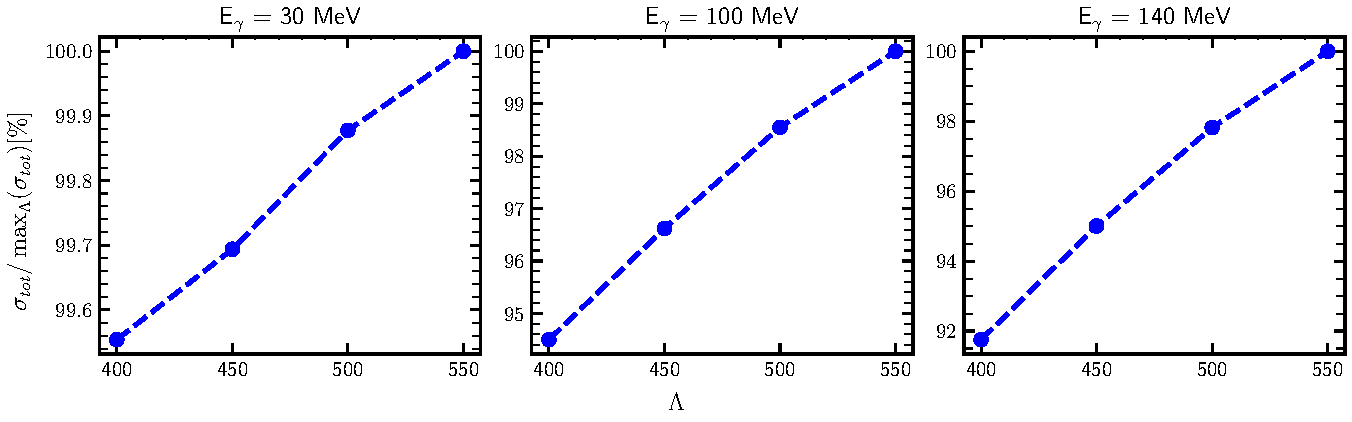
\includegraphics[width=0.95\textwidth]{Figures_De/TOTAL_CROSSSECTION_cutoff.pdf}
        \end{center}
        \caption{Total cross section of the deuteron photodisintegration
        process (normalized to the maximal cross section among all $\Lambda$)
        as a dependance on the cutoff parameter $\Lambda$ 
        for three photon energy E$_\gamma$ values: 30, 100 and 140 MeV.}
        \label{Cutoff_dep}
        \end{figure}

    Another theoretical uncertainty comes from the choice of the cutoff parameter's value 
    of regulator described in chapter \tmp{??????? put link}.

    The free parameters of \gls{sms} potential have been obtained from data for 
    % According to \cite{reinkrebs2018}, where the \gls{sms} potential was presented,
   four values of the cutoff parameter $\Lambda$:
   \SIlist[list-units = single]{400;450;500;550}{\mev} \cite{reinkrebs2018}.
   Using each of whese values, one obtains different predictions which off course can further differ 
   from actual (experimental) value. Therefore the choice of $\Lambda$ value
   may affect a quality of the prediction.

    To study that I also use the same four values of the $\Lambda$ parameter,
    obtaining in that way four predictions each time.
    That is exemplified in \fig{Cutoff_dep}  for the deuteron photodisintegration cross section for the
    photon's energy $E_\gamma = \SIlist{30;100;140}{\mev}$.
    The \gls{sms} model at \gls{n4lo+} is used.
    % Comparison of predictions obtained with different values of the 
    % cutoff parameter $\Lambda$ is presented on the Fig.~\ref{Cutoff_dep}.
    Each subfigure shows a predictions for the total cross section as 
    a function of the cutoff parameter,
    normalized to the maximum value among all cross sections
    obtained with various $\Lambda$.
    As we can see, for that observable
    there is almost linear dependance with positive linearity coefficient value:
    with higher $\Lambda$ the cross section value increases as well.
    Note that with higher photon's energy,
    the cutoff dependance becomes stronger: for $E_\gamma=\SI{30}{\mev}$
    the maximal difference between predictions is around \SI{0.5}{\percent} while
    for \SI{140}{\mev} it increases to more than \SI{8}{\percent}. This results are
    generally within our expectations that our model works better at
    smaller energies
    and is less sensitive to the $\Lambda$ value. LEt us remind that $\Lambda$ 
    governs the behavior of the potential at small internucleon distances and only higher energy transfer probes that distances. 



    \subsection*{Other theoretical uncertainies}

    There are obviously more sources of theoretical uncertainties. 
    Our model has a number of either intrinsic limitations in precision or 
    some simplifications which may be improved with further developments of the model.
    
    \paragraph{Nuclear currents}
    At the moment, our model is limited to a single nucleon current, which may not be sufficient to accurately describe the processes under consideration.  This limitation will be further discussed and confirmed in
    Chapter~\ref{chap:results}. To address this issue, we utilize the Siegert theorem, which enables us to
    incorporate some contributions from the two-nucleon current, although it is not yet complete. It is worth noting
    that the incorporation of the two-nucleon current can significantly affect the predicted observables, as it
    includes additional physical effects that are not accounted for in the single nucleon current. Therefore, the
    ongoing development of a complete two-nucleon current in our model
    is of great importance to improve the accuracy of our predictions.

    \paragraph{Nonrelativistic approach}
    All the results presented here does not include relativistic corrections.
    At the lower energies the relativistic contribution might not be crucial,
    but at the region with higher energy we may see a lack of precision.
    This well be also confirmed and discussed regarding the total cross section
    for the deuteron photodisintegration \fig{TOTAL_CROSS}.
    
    \paragraph{Uncertainties in the potential free parameters}
    \tmp{????}

    \paragraph{Uncertainties from the numerical method}
    All the results include numerical calculations,
    so we can come up with a lot of places were numerical methods with limited 
    precision come into the scene. 
    Our approach is based on the partial wave decomposition which
    supposes that limited numer of partial waves are included 
    (usually for 2N scattering we use $j^{max}=4$ which corresponds to 18 partial waves).
    For 3N calculations we use $J^{max}=5$ which corresponds to 40 partial waves.
    In addition, we with some 
    grid of points which is used for the calculation of potential, wave function, numerical integration etc. 
    The choice of grid affect
    a final results' precision. 
    % The same grid is also used for numerical integration
    % (e.g. in \eq{integral2}) where the final integral is also dependant on the points.
    Usually, we use a grid {\tmp{ of ... values}} which was proven to make resulting
    uncertainty small.

    \paragraph{Model choice}
    We focus on the \gls{sms} potential, but using another model of interaction 
    leads to different predictions. That difference is also a theoretical uncertainty thus
    we use predictions obtained with AV18 model in order to compare these predictions.
    The AV18 model is a widely used and well-established model of nuclear interaction,
    which has been extensively tested and benchmarked against experimental data. By comparing
    the predictions obtained from the SMS potential with those obtained from the AV18 model,
    we can assess the robustness of our results and determine the extent to which they depend
    on the choice of the interaction model. This comparison also helps to identify the strengths
    and weaknesses of each model and provides insights into the underlying physics of nuclear interactions.

    \paragraph{Machine precision}
    % Finally every computer calculations include limited numerical machine precision which
    % can be noticeable for a complex calculations. We perform our calculation via CPU machine 
    % were particular choice of the processor and memory card may lead to numerical uncertainty.
    % Nevertheless this uncertainty is much smaller then other discussed above. 

    Finally, it should be noted that every computer calculation includes limited numerical machine precision which
    can be noticeable for complex calculations. We perform our calculations via CPU machine, where the particular
    choice of the processor and memory card may lead to numerical uncertainty. However, we have found that this
    uncertainty is much smaller than the uncertainties discussed above, and its impact on our results is
    negligible. We have taken great care to ensure that our calculations are performed using appropriate numerical
    methods and sufficient computational resources to minimize any numerical errors that may arise. 
